\chapter{Planes in Space}

\begin{center}
    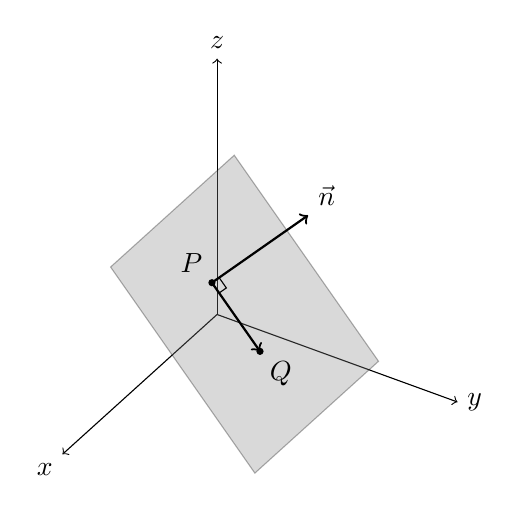
\begin{tikzpicture}[x={({cos(20)},{-sin(20)},0)},z={({-sin(40)},{-cos(40)},0)},scale=0.65]
        %draw x, y and z axis
        \draw[->] (0, 0, 0) -- (5, 0, 0);
        \draw[->] (0, 0, 0) -- (0, 5, 0);
        \draw[->] (0, 0, 0) -- (0, 0, 5);
        %draw a 3d sloped plane
        \draw[-, fill=gray, opacity=0.3] (1, 4, 1) -- (1, 4, 5) -- (4, 1, 5) -- (4, 1, 1) -- cycle;
        % label x, y and z axis
        \node[right] at (5, 0, 0) {$y$};
        \node[above] at (0, 5, 0) {$z$};
        \node[below left] at (0, 0, 5) {$x$};

        \fill (1.5,2.5,2.5) circle (0.2em) node [above left] {$P$};
        \fill (2.5,1.5,2.5) circle (0.2em) node [below right] {$Q$};
        \draw [->, thick] (1.5,2.5,2.5) -- (2.5,1.5,2.5);
        \draw [->, thick] (1.5,2.5,2.5) -- (3.5,4.5,2.5) node [above right] {$\vec{n}$};
        \draw (1.65,2.65,2.5) -- (1.8,2.5,2.5) -- (1.65,2.35,2.5);
    \end{tikzpicture}
\end{center}

To find the equation of a plane in space, we need a point $P(x_1, y_1, z_1)$ on
the plane and a vector $\vec{n} = \langle a, b, c \rangle$ that is orthogonal
to the plane, called the \textbf{normal vector} of the plane.

For any point $Q(x, y, z)$ on the plane, the vector $\overrightarrow{PQ}$ is
orthogonal to $\vec{n}$, that is,
\begin{align*}
    \overrightarrow{PQ} \cdot \vec{n}                                       & = 0 \\
    \langle x - x_1, y - y_1, z - z_1 \rangle \cdot \langle a, b, c \rangle & = 0 \\
    a(x - x_1) + b(y - y_1) + c(z - z_1)                                    & = 0
\end{align*}
This equation is called the \textbf{standard form} of the equation of the plane. Regrouping the terms, we obtain the \textbf{general form} of equation of the plane. \[ax + by + cz + d = 0\] where $d = -ax_1 - by_1 - cz_1$.

\newpage
\noindent\textbf{Example 1. } Find the
equation of the plane that passes through the point $P(4, 5, -7)$ and is
perpendicular to the vector $\vec{n} = \hat{\jmath}$.
\begin{align*}
    \vec{n}                        & = \langle 0, 1, 0 \rangle \\
    0(x - 4) + 1(y - 5) + 0(z + 7) & = 0                       \\
    y - 5                          & = 0                       \\
    y                              & = 5
\end{align*}
\noindent\textbf{Example 2. } Find the
equation of the plane that passes through the point $P(0, 7, 0)$ and is
perpendicular to the vector $\vec{n} = 3\hat{\imath} + 8\hat{k}$.
\begin{align*}
    \vec{n}                        & = \langle 3, 0, 8 \rangle \\
    3(x - 0) + 0(y - 7) + 8(z - 0) & = 0                       \\
    3x + 8z                        & = 0
\end{align*}
\noindent\textbf{Example 3. } Given three points $(0, 0, 0)$, $(2, 0, 7)$, and $(-2, -1, 7)$ in space, find the equation of the plane that passes through these points.
\begin{align*}
    \vec{u} & = \langle 2 - 0, 0 - 0, 7 - 0 \rangle                                                  \\
            & = \langle 2, 0, 7 \rangle                                                              \\
    \vec{v} & = \langle -2 - 0, -1 - 0, 7 - 0 \rangle                                                \\
            & = \langle -2, -1, 7 \rangle                                                            \\
    \vec{n} & = \vec{u} \times \vec{v}                                                               \\
            & = \begin{vmatrix}
                    \hat{\imath} & \hat{\jmath} & \hat{k} \\
                    2            & 0            & 7       \\
                    -2           & -1           & 7
                \end{vmatrix}                            \\
            & = \begin{vmatrix}
                    0  & 7 \\
                    -1 & 7
                \end{vmatrix}\hat{\imath} - \begin{vmatrix}
                                                2  & 7 \\
                                                -2 & 7
                                            \end{vmatrix}\hat{\jmath} + \begin{vmatrix}
                                                                            2  & 0  \\
                                                                            -2 & -1
                                                                        \end{vmatrix}\hat{k}         \\
            & = (0(7) - 7(-1))\hat{\imath} - (2(7) - (-2)(7))\hat{\jmath} + (2(-1) - (-2)(0))\hat{k} \\
            & = 7\hat{\imath} - 28\hat{\jmath} - 2\hat{k}                                            \\
            & = \langle 7, -28, -2 \rangle
\end{align*}
\begin{align*}
    7(x - 0) - 28(y - 0) - 2(z - 0) & = 0 \\
    7x - 28y - 2z                   & = 0
\end{align*}
\newpage
\noindent\textbf{Example 4. } Find the equation of the plane that passes through $(4, 2, 1)$, $(-1, 8, 8)$ and is parallel to $z$-axis.
\begin{align*}
    \vec{v} & = \langle -1 - 4, 8 - 2, 8 - 1 \rangle                                           \\
            & = \langle -5, 6, 7 \rangle                                                       \\
    \vec{n} & = \vec{v} \times \hat{k}                                                         \\
            & = \begin{vmatrix}
                    \hat{\imath} & \hat{\jmath} & \hat{k} \\
                    -5           & 6            & 7       \\
                    0            & 0            & 1
                \end{vmatrix}                      \\
            & = \begin{vmatrix}
                    6 & 7 \\
                    0 & 1
                \end{vmatrix}\hat{\imath} - \begin{vmatrix}
                                                -5 & 7 \\
                                                0  & 1
                                            \end{vmatrix}\hat{\jmath} + \begin{vmatrix}
                                                                            -5 & 6 \\
                                                                            0  & 0
                                                                        \end{vmatrix}\hat{k}   \\
            & = (6(1) - 7(0))\hat{\imath} - (-5(1) - 7(0))\hat{\jmath} + (-5(0) - 6(0))\hat{k} \\
            & = 6\hat{\imath} + 5\hat{\jmath}                                                  \\
            & = \langle 6, 5, 0 \rangle
\end{align*}
\vspace{-3.5em}
\begin{align*}
    6(x - 4) + 5(y - 2) + 0(z - 1) & = 0 \\
    6x + 5y - 34                   & = 0
\end{align*}
\noindent\textbf{Example 5. } Find the equation of the plane such that the point $(2, 0, 1)$ and the line $\dfrac{x}{2} = \dfrac{y-4}{-1} = \dfrac{z}{1}$ is on the plane.
~\\
When $x = 0$, $y = 4$ and $z = 0$, hence the point $(0, 4, 0)$ is on the plane.
\begin{align*}
    \vec{v} & = \langle 2 - 0, 0 - 4, 1 - 0 \rangle                                              \\
            & = \langle 2, -4, 1 \rangle                                                         \\
    \vec{n} & = \langle 2, -1, 1 \rangle \times \langle 2, -4, 1 \rangle                         \\
            & = \begin{vmatrix}
                    \hat{\imath} & \hat{\jmath} & \hat{k} \\
                    2            & -1           & 1       \\
                    2            & -4           & 1
                \end{vmatrix}                        \\
            & = \begin{vmatrix}
                    -1 & 1 \\
                    -4 & 1
                \end{vmatrix}\hat{\imath} - \begin{vmatrix}
                                                2 & 1 \\
                                                2 & 1
                                            \end{vmatrix}\hat{\jmath} + \begin{vmatrix}
                                                                            2 & -1 \\
                                                                            2 & -4
                                                                        \end{vmatrix}\hat{k}     \\
            & = (-1(1) - 1(-4))\hat{\imath} - (2(1) - 2(1))\hat{\jmath} + (2(-4) - 2(-1))\hat{k} \\
            & = -3\hat{\imath} + 0\hat{\jmath} + (-6)\hat{k}                                     \\
            & = \langle -3, 0, -6 \rangle
\end{align*}
\vspace{-3.5em}
\begin{align*}
    -3(x - 2) + 0(y - 0) - 6(z - 1) & = 0 \\
    -3x - 6z + 12                   & = 0
\end{align*}
\newpage
\noindent\textbf{Example 6. } Find the equation of the plane that passes through the points $(3, 4, 1)$ and $(3, 1, -7)$ and is perpendicular to the plane $8x + 9y + 3z  = 13$.
~\\\\
The normal vector of the plane is $\langle 8, 9, 3 \rangle$. Since the target plane is perpendicular to the given plane, the normal vector of the given plane is parallel to the target plane.
\begin{align*}
    \vec{u} & = \langle 8, 9, 3 \rangle                                                          \\
    \vec{v} & = \langle 3 - 3, 1 - 4, -7 - 1 \rangle                                             \\
            & = \langle 0, -3, -8 \rangle                                                        \\
    \vec{n} & = \vec{u} \times \vec{v}                                                           \\
            & = \begin{vmatrix}
                    \hat{\imath} & \hat{\jmath} & \hat{k} \\
                    8            & 9            & 3       \\
                    0            & -3           & -8
                \end{vmatrix}                        \\
            & = \begin{vmatrix}
                    9  & 3  \\
                    -3 & -8
                \end{vmatrix}\hat{\imath} - \begin{vmatrix}
                                                8 & 3  \\
                                                0 & -8
                                            \end{vmatrix}\hat{\jmath} + \begin{vmatrix}
                                                                            8 & 9  \\
                                                                            0 & -3
                                                                        \end{vmatrix}\hat{k}     \\
            & = (9(-8) - 3(-3))\hat{\imath} - (8(-8) - 3(0))\hat{\jmath} + (8(-3) - 9(0))\hat{k} \\
            & = -63\hat{\imath} + 64\hat{\jmath} - 24\hat{k}                                     \\
            & = \langle -63, 64, -24 \rangle
\end{align*}
\vspace{-3.5em}
\begin{align*}
    -63(x - 3) + 64(y - 4) - 24(z - 1) & = 0 \\
    -63x + 64y - 24z - 43              & = 0
\end{align*}
